\documentclass[a4paper, top=10mm]{article}
%for writing from the top
\usepackage{fullpage}
%for math
\usepackage{amsmath}
\usepackage{mathrsfs}
\usepackage{amsthm}
%for images
\usepackage{graphicx}
%for color
\usepackage{xcolor}
%for title
\title{\textbf{\huge{Best Power of Two}}}
\author{Enigma n\textsuperscript{o}5}
\date{19\textsuperscript{th} December 2024}

\newtheorem*{hint}{Hint}

\addtolength{\voffset}{-2cm}
\addtolength{\textheight}{5cm}


\begin{document}
	\maketitle
	
	What is the smallest power of two that does not feature a 0, 1, 2, 4 or 8 in its decimal representation?
	
	\begin{center}
		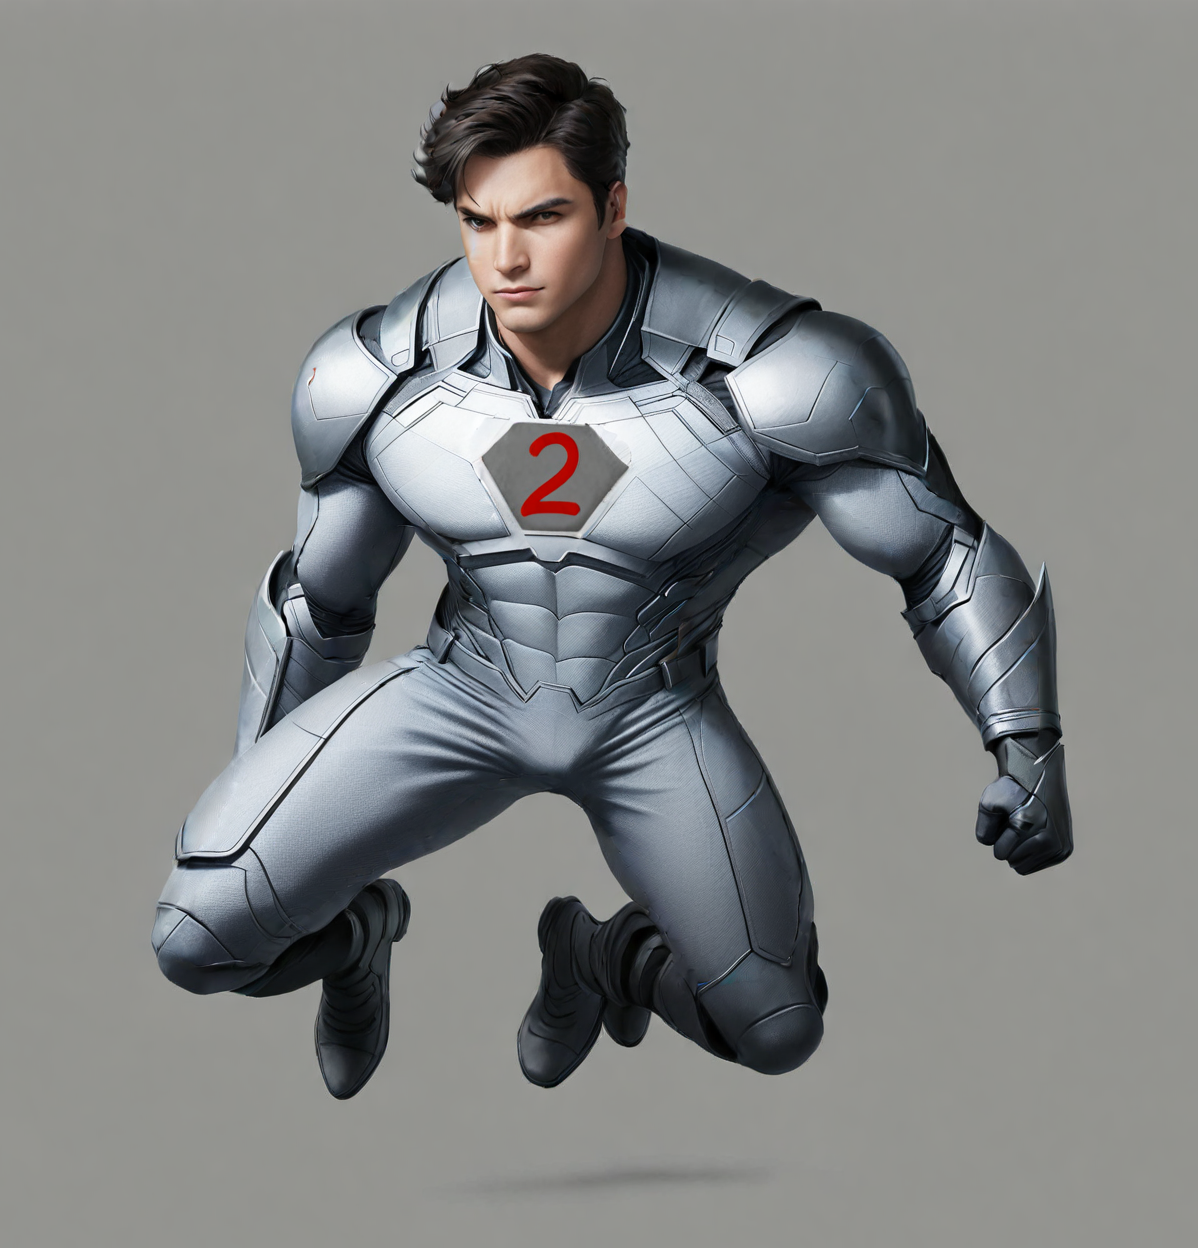
\includegraphics[width=\linewidth]{05best_power2bis.png}\\
		Mr. Powertwo
	\end{center}
	
	\underline{Note:} It could be the only power of two that does not feature any of these digits, but I have not proved it.
	
	% Answer: 50%
	
\end{document}